\section{Part 3: Non-linear Kalman Filters}
\subsection{Essential Background III}

\subsubsection{The square root of a matrix}
\begin{frame}{Essential Background III---The square root of a matrix}

The non-linear Kalman Filter requires prior knowledge of the Derivatives (EKF) and Matrix Square Root (UKF).

\vspace{10pt}
A matrix \(\mathbf{B}\) is a square root of a matrix \(\mathbf{A}\) if:
\[
\mathbf{A} = \mathbf{B}\mathbf{B} 
\]

The equation above can have several possible solutions, and there are different computation methods for finding the square root of a matrix.

\vspace{10pt}
The Unscented Kalman Filter employs an Unscented Transform that requires a square root computation of a covariance matrix. 

\vspace{10pt}
As covariance matrices are positive and semi-definite, we can use \textbf{Cholesky decomposition (or Cholesky factorization)} for the computation of a covariance matrix square root.

\end{frame}

%--------------------------
\subsubsection{Cholesky decomposition}
\begin{frame}{Cholesky decomposition}
\vspace{-7pt}
The Cholesky decomposition is a decomposition of a positive definite matrix into a product of a lower triangular matrix and its transpose.

If a matrix \(\mathbf{A}\) is positive definite:
\[
\mathbf{A} = \mathbf{L} \mathbf{L}^T 
\]

The lower triangular matrix is a square matrix where all the values above the diagonal are zero:
\vspace{-7pt}
\[
\begin{bmatrix}
a_{11} & a_{12} & a_{13} & a_{14} \\
a_{21} & a_{22} & a_{23} & a_{24} \\
a_{31} & a_{32} & a_{33} & a_{34} \\
a_{41} & a_{42} & a_{43} & a_{44}
\end{bmatrix}
=
\begin{bmatrix}
l_{11} & 0 & 0 & 0 \\
l_{21} & l_{22} & 0 & 0 \\
l_{31} & l_{32} & l_{33} & 0 \\
l_{41} & l_{42} & l_{43} & l_{44}
\end{bmatrix}
\begin{bmatrix}
l_{11} & l_{12} & l_{13} & l_{14} \\
0 & l_{22} & l_{23} & l_{24} \\
0 & 0 & l_{33} & l_{34} \\
0 & 0 & 0 & l_{44}
\end{bmatrix}
\]

If matrix \(\mathbf{A}\) is positive semi-definite, then the diagonal entries of \(\mathbf{L}\) are allowed to be zero.

\textbf{Cholesky decomposition algorithm:}

- Diagonal elements of \(\mathbf{L}\):
\[
l_{vv} = \sqrt{a_{vv} - \sum_{u<v} l_{vu}^2}
\]

- Off-diagonal elements of \(\mathbf{L}\):
\[
l_{tv} = \frac{1}{l_{vv}} \left( a_{tv} - \sum_{u<v} l_{tu} l_{vu} \right)
\]

First, find the elements of the first row of \(\mathbf{L}\), then find the elements of the second row of \(\mathbf{L}\), and then find the elements of the third row of \(\mathbf{L}\). Continue the process until you reach the final row.

\textcolor{blue}{Implementation: \textbf{Python}: L = np.linalg.cholesky(A), \textbf{Matlab}: L = chol(A)}    
\end{frame}


%---------------------------------
\subsection{Non-linearity Problem}

\begin{frame}{Non-linearity Problem}
    Necessary background on what are the non-linear systems, and why does the standard Linear Kalman Filter fail with non-linear systems?

    We need to distinguish between two types of non-linearities:

    \begin{itemize}
        \item State-to-measurement non-linear relation
        \item Non-linear system dynamics
    \end{itemize}

We must treat each type of non-linearity separately and then combine them.
\end{frame}

%---------------------------------
\subsubsection{Example – linear system}
\begin{frame}{Example – linear system}
\begin{columns}
        \column{0.5\textwidth}

        \begin{itemize}
            \item Assume an air balloon that can move only upwards or downwards with constant
        acceleration dynamics. We are interested in estimating the balloon altitude.
        
        \item Since the balloon system dynamic model is linear, it can be described as:
        \vspace{-5pt}
        \[
\mathbf{\hat{x}}_{n+1,n} = F \mathbf{\hat{x}}_{n,n}
\]
\[
\begin{bmatrix} \hat{x}_{n+1,n} \\ \hat{\dot{x}}_{n+1,n} \\ \hat{\ddot{x}}_{n+1,n} \end{bmatrix} = \begin{bmatrix} 1 & \Delta t & 0.5\Delta t^2 \\ 0 & 1 & \Delta t \\ 0 & 0 & 1 \end{bmatrix} \begin{bmatrix} \hat{x}_{n,n} \\ \hat{\dot{x}}_{n,n} \\ \hat{\ddot{x}}_{n,n} \end{bmatrix}
\]

\item The balloon altitude is measured by the radar located beneath the balloon.
\item The radar measurement error distribution is Gaussian.

\item The radar sends an EM pulse; the pulse is reflected from the balloon and received by the radar. The radar measures the time elapsed
between pulse transmission and reception. Since the pulse travels with the speed of light, we can calculate the target range (i.e., balloon altitude) as $x = t\times{c}/{2}$
\end{itemize}
        \column{0.5\textwidth}
        \begin{figure}
            \centering
            
\includegraphics[width=0.2\linewidth]{Figures//Background3/Ballon_LinearSystem.png}
            \caption{Balloon altitude measurement using radar}
        \end{figure}
    \begin{itemize}
        \item Let us construct the observation matrix $\mathbf{H}$.
        \[
        z_n = \mathbf{H} x_n \quad \text{with} \quad \mathbf{H} = \begin{bmatrix} \frac{c}{2} \end{bmatrix} 
        \]
        \item The dependency between the measured value ($z_n$--elapsed time) and the estimated value
        ($x_n$--balloon altitude) is linear.

        \item However, what happens to the estimation uncertainty? Is it still Gaussian?

    \end{itemize}
        
\end{columns}
\end{frame}
%---------------------------------
\begin{frame}{Example – linear system}
The following chart depicts the dependency between the elapsed time and the balloon altitude.
\vspace{-10pt}
\begin{figure}
    \centering
    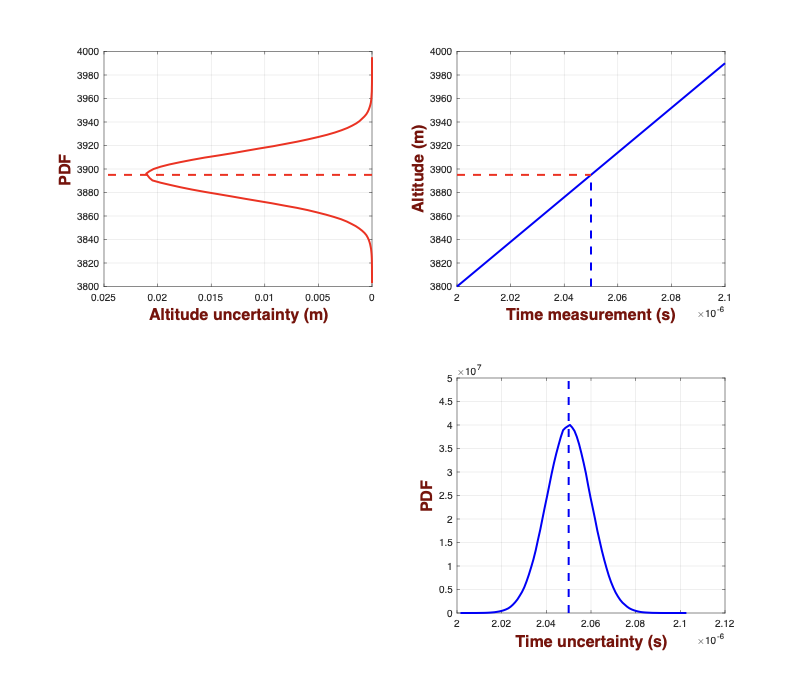
\includegraphics[width=0.6\linewidth]{Figures//Background3/Ballon_LinearDynamics_Results.png}
    \vspace{-15pt}
    \caption{The dependency between the elapsed time and the balloon altitude: the distribution of measurement error (uncertainty) on the bottom plot and the state estimation error (uncertainty) on the left plot.}
\end{figure}
Since the dependency between the measured value and the estimated value is linear, the estimated value uncertainty is also Gaussian!

\texttt{\tiny [Code: Non-linear KF/Ballon\_LinearDynamics.m]}
\end{frame}
%---------------------------------
\subsubsection{Example – State-to-measurement non-linear relation}
\begin{frame}{Example – State-to-measurement non-linear relation}
This example presents the first type of non-linearity: state-to-measurement relation.
\begin{columns}
        \column{0.5\textwidth} 
        \begin{itemize}

            \item Like the earlier example, we are interested in measuring the balloon altitude, while the balloon system dynamic model is linear.
            
            \item The balloon altitude is measured by the optical sensor that is located aside, using the target angle, with Gaussian measurement error distribution.
            
            \item The distance $d$ between the sensor and the balloon nadir is known. 

            \begin{figure}
                \centering
                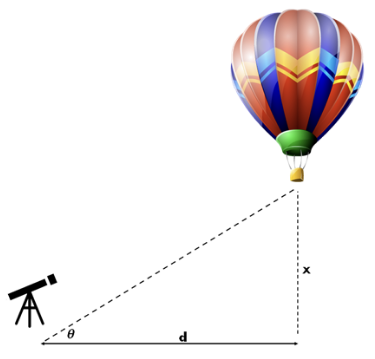
\includegraphics[width=0.55\linewidth]{Figures//Background3/Ballon_Optical sensor_nonlinear.png}
                \vspace{-8pt}
                \caption{Balloon altitude measurement using an optical sensor.}
            \end{figure}
        \end{itemize}
        
        \column{0.5\textwidth}
        \begin{itemize}
            \item The balloon altitude can be calculated by using a trigonometric function:
            \begin{equation*}
            x = d \cdot \tan(\theta)
            \end{equation*}
            \vspace{-10pt}
            \begin{itemize}
                \item $x$ is the balloon altitude
                \item $d$ is the distance between the sensor and the balloon nadir
                \item $\theta$ is the balloon's elevation angle
            \end{itemize}

        \item As tangent function is non-linear, we can’t construct the observation matrix $\mathbf{H}$!
        \item recall: for a linear system, the measurement equation is
        \[
        \mathbf{z}_n = \mathbf{H} \mathbf{x}_n + \mathbf{v}_n
        \]
        \item For non-linear state-to-measurement relation system, the observation matrix $\mathbf{H}$ is a function of $x$, with measurement eq.:
        \[
        \mathbf{z}_n = \mathbf{h}(\mathbf{x}_n, \mathbf{v}_n)  
        \]
        In this example, $\theta = \tan^{-1}\frac{x}{d}$
        \end{itemize}
            
\end{columns}
\end{frame}
%---------------------------------
\begin{frame}{Example – State-to-measurement non-linear relation}
\begin{figure}
    \centering
    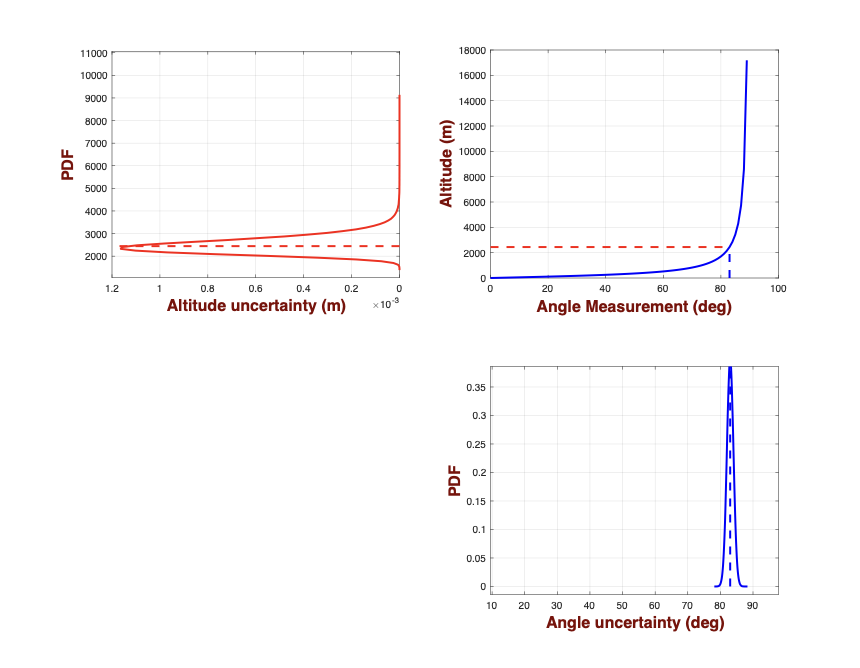
\includegraphics[width=0.5\linewidth]{Figures//Background3/Ballon_NonLinearDynamics_Results.png}
    \vspace{-15pt}
    \caption{Non-linear System: The dependency between the measured angle and the balloon altitude, with the distribution of measurement error (uncertainty) on the bottom plot and the state estimation error (uncertainty) on the left plot.}
    \end{figure}
    The altitude uncertainty distribution is not Gaussian! It also changes its shape at different measurement points.
    
    The Kalman Filter algorithm assumes that the distribution of all random variables is Gaussian. For non-linear systems, this assumption does not hold anymore. The algorithm is not stable and yields significant estimation errors.

\texttt{\tiny [Code: Non-linear KF/Ballon\_State2MeasurementUncertainty.m]}

\end{frame}
%---------------------------------
\subsubsection{Example – Non-linear system dynamics}
\begin{frame}{Example – Non-linear system dynamics}
        This example presents the second type of non-linearity: non-linear system dynamics.   
\begin{columns}
        \column{0.5\textwidth}
        \begin{itemize}
            \item Assume an ideal gravity pendulum that consists of a body with mass $m$ hung by a string with length $L$ from fixed support - the pendulum swings back and forth at a constant amplitude. We want to estimate the angle $\theta$ (radians) from the vertical to the pendulum.
        \end{itemize}
        \vspace{-8pt}
        \begin{figure}
            \centering
            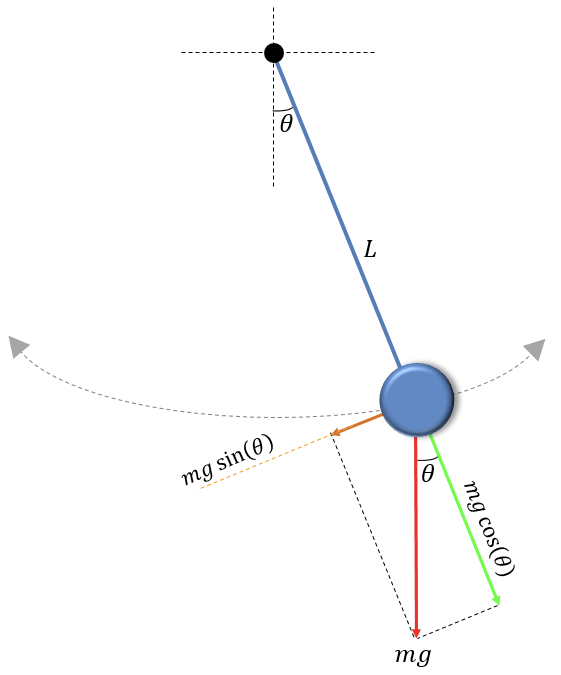
\includegraphics[width=0.50\linewidth]{Figures//Background3/Pendulum.png}
            \vspace{-8pt}
            \caption{Pendulum}
            \vspace{-10pt}
        \end{figure}
         \begin{itemize}
     \item According to Newton’s second law, the sum of forces on the object equals $F=ma$.
     \end{itemize}
 \column{0.5\textwidth}
 \begin{itemize}
     \item The force applied to the pendulum equals $$F = -mg\sin(\theta) = ma \Rightarrow a = -g\sin(\theta)$$
     \item The arc length $s$ that corresponds to angle $\theta$ is
    $$s=L\theta$$
     \item The pendulum velocity equals
     $$v = \frac{ds}{dt}=L\frac{d\theta}{dt}$$
     \item The pendulum acceleration equals
     $$a = \frac{d^2s}{dt^2}=L\frac{d^2\theta}{dt^2} = -g\sin{\theta}$$
     \item Thus, the differential equation that describes the pendulum movement is a second-order homogeneous differential equation:
     \vspace{-10pt}
     $$L\frac{d^2\theta}{dt^2} = -g\sin{\theta}$$
 \end{itemize}
\end{columns}
\end{frame}
%---------------------------------
\begin{frame}{Example – Non-linear system dynamics}
\begin{columns}
        \column{0.5\textwidth} 
        \vspace{-15pt}
        
        \textbf{Dynamic model of the system:}
The state vector of the pendulum is in the form of the following:
\[
\mathbf{x}_n =
\begin{bmatrix}
\theta_n \\
\dot{\theta}_n
\end{bmatrix}
\]
\vspace{-10pt}
\begin{itemize}
    \item $\theta_n$ is the pendulum angle at time $n$
    \item $\dot{\theta}_n$ is the pendulum angular velocity at time $n$
\end{itemize}
\[
\begin{aligned}
    \hat{\theta}_{n+1, n} &= \hat{\theta}_{n, n} + \hat{\dot{\theta}}_{n, n}\Delta t \\
    \hat{\dot{\theta}}_{n+1, n} &= \hat{\dot{\theta}}_{n, n} + \hat{\ddot{\theta}}_{n, n}\Delta t = \hat{\dot{\theta}}_{n, n} - \frac{g}{L} \sin(\hat{\theta}_{n, n}) \Delta t
\end{aligned}
\]

The dynamic model is not linear. For a linear system, the general form of the state extrapolation equation in a matrix notation is:
\[
\hat{\mathbf{x}}_{n+1, n} = \mathbf{F} \hat{\mathbf{x}}_{n, n} + \mathbf{G} u_n + \mathbf{w}_n \quad
\]
        For the non-linear system dynamics, the state transition matrix $\mathbf{F}$ is a function of $\mathbf{x}$ and $\mathbf{u}$. Therefore, the state extrapolation equation looks as:
\[
\hat{\mathbf{x}}_{n+1, n} = \mathbf{f}(\hat{\mathbf{x}}_{n, n}, \mathbf{u}_n, \mathbf{w}_n)
\]
        \column{0.5\textwidth}
In this example:
\[
f(\hat{\mathbf{x}}_{n+1, n}) =
\begin{bmatrix}
\hat{\theta}_{n, n} + \hat{\dot{\theta}}_{n, n} \Delta t \\
\hat{\dot{\theta}}_{n, n} - \frac{g}{L} \sin(\hat{\theta}_{n, n}) \Delta t
\end{bmatrix}
\]

The measurement equation depends on the measured parameter. Let's review two cases:
\textbf{Case 1 - Measured parameter is pendulum angle $\theta$:} In this case, the measurement equation looks like:
\vspace{-8pt}
\[
\theta_{n,\text{measured}} =
\begin{bmatrix}
1 & 0
\end{bmatrix}
\begin{bmatrix}
\theta_n \\
\dot{\theta}_n
\end{bmatrix}
\]
The above equation is in the form of: $\mathbf{z}_n = \mathbf{H}\mathbf{x}_n$. Therefore, the state-to-measurement relation (the first type of non-linearity) is linear.

\textbf{Case 2 - Measured parameter is the pendulum $x$-position:} In this case, the measurement equation is:
\vspace{-8pt}
\[
x_{n,\text{measured}} = L\sin(\theta_n)
\]
which is in the form of: $\mathbf{z}_n = \mathbf{h}(\mathbf{x}_n)$. Therefore, the state-to-measurement relation is non-linear.

\end{columns}
\end{frame}
%---------------------------------